\section{Przypadki użycia}

Wszelkie przypadki użycia posiadają warunek poprawnego przejścia scenariusza pierwszego (UC1 Autoryzacja użytkownika).

\subsection{Autoryzacja użytkownika} 
\begin{adjustwidth}{2em}{0pt}
Nazwa: UC1 Autoryzacja użytkownika \\
Opis: Proces logowania się pracownika \\
Aktorzy: Użytkownik \\
Warunki początkowe: 
\begin{itemize}
\item Istniejące konto w systemie 
\end{itemize}
Warunki końcowe: 
\begin{itemize}
\item Dostęp do systemu 
\end{itemize}
Scenariusz główny:
\begin{enumerate}
\item Aktor wprowadza swoje login i hasło
\item System sprawdza zapytanie
\item System wyświetla ekran powitalny
\end{enumerate}
Scenariusz alternatywny - błędne dane: 
\begin{enumerate}
\item Aktor wprowadza swoje login i hasło
\item System uznaje zapytanie za błędne
\item System wyświetla ekran informujący o błędnym loginie lub haśle 
\end{enumerate}
\end{adjustwidth}

\subsection{Dodanie/edycja profilu użytkownika}
\begin{adjustwidth}{5em}{0pt}
Nazwa: UC2 Dodanie/edycja profilu użytkownika \\
Opis: Proces dodania/edycji profilu dla pracownika \\
Aktorzy: HR \\
Warunki początkowe:
\begin{itemize}
\item Dokument z informacjami dotyczącymi pracownika
\end{itemize}
Warunki końcowe: 
\begin{itemize}
\item Uaktualniony profil pracownika
\end{itemize}
Scenariusz główny:
\begin{enumerate}
\item Aktor otwiera formularz profilu pracownika
\item Aktor uzupełnia/zmienia wybrane pola
\item Aktor potwierdza zmiany odpowiednim przyciskiem
\item System zapisuje w bazie danych nowe dane
\item System wyświetla ekran poglądowy z nowym profilem użytkownika
\end{enumerate}
Scenariusz alternatywny - walidacja danych: 
\begin{enumerate}
\item Jak a-c w scenariuszu głównym
\item System wykrywa błędnie wpisane dane 
\item System zwraca formularz z zaznaczonymi błędnymi polami
\end{enumerate}
Scenariusz alternatywny - utrata łączności: 
\begin{enumerate}
\item Jak a-c w scenariuszu głównym
\item System ma problem z łącznością 
\item System wyświetla formularz, wraz z informacją o nie zapisaniu danych spowodowanych problemem łączności
\end{enumerate}
Scenariusz alternatywny - kolizja transakcji: 
\begin{enumerate}
\item Jak a-c w scenariuszu głównym
\item System wykrywa błąd transakcji (np. zakleszczenie)
\item System wyświetla formularz, wraz z prośbą o ponowienie zapytania
\end{enumerate}
\end{adjustwidth}

\subsection{Usuwanie profilu użytkownika}
\begin{adjustwidth}{5em}{0pt}
Nazwa: UC3 Usuwanie profilu użytkownika \\
Opis: Proces usuwania profilu dla pracownika \\
Aktorzy: HR lub Administrator \\
Warunki początkowe:
\begin{itemize}
\item Informacja o koncie do usunięcia
\end{itemize}
Warunki końcowe: 
\begin{itemize}
\item Zaktualizowana baza danych pozbawiona nieporządanego konta
\end{itemize}
Scenariusz główny:
\begin{enumerate}
\item Aktor otwiera listę użytkowników
\item Aktor wybiera opcje usunięcie konta przy nazwisku
\item System usuwa rekord z informacjami o użytkowniku
\item System wyświetla nową listę użytkowników
\end{enumerate}
Scenariusz alternatywny - błąd usuwania: 
\begin{enumerate}
\item Jak a-b w scenariuszu głównym
\item System wykrywa błąd podczas usuwania rekordu
\item System zwraca pierwotną listę z informacją z błędem usuwania
\end{enumerate}
\end{adjustwidth}

\subsection{Zmiana praw dostępu}
\begin{adjustwidth}{5em}{0pt}
Nazwa: UC4 Zmiana praw dostępu \\
Opis: Proces zmiany uprawnień użytkownika do określonych modułów. \\
Aktorzy: Administrator \\
Warunki początkowe:
\begin{itemize}
\item Dotychczas nadane prawa 
\end{itemize}
Warunki końcowe: 
\begin{itemize}
\item Uaktualniony profil z nowymi rolami
\end{itemize}
Scenariusz główny: 
\begin{enumerate}
\item Aktor wybiera z listy edytowane konto użytkownika
\item System wyświetla detale profilu użytkownika
\item Aktor wybiera odpowiednią opcję ról i zatwierdza
\item System zmienia rekord dotyczący ról dla danego konta
\item System zwraca widok profilu użytkownika z nowymi prawami dostępu
\end{enumerate}
Scenariusz alternatywny - błąd zmiany : 
\begin{enumerate}
\item Jak a-c w scenariuszu głównym
\item System wykrywa kolizję lub błąd połączenia
\item System wyświetla detale profilu użytkownika wraz z kodem błędu, który wystąpił
\end{enumerate}
\end{adjustwidth}

\subsection{Edycja zwierzchnictwa}
\begin{adjustwidth}{5em}{0pt}
Nazwa: UC5 Edycja zwierzchnictwa \\
Opis: Proces zmiany hierarchii drzewa struktury firmy. \\
Aktorzy: Administrator lub HR \\
Warunki początkowe:
\begin{itemize}
\item Dokument dotyczący hierarchii firmy
\end{itemize}
Warunki końcowe:
\begin{itemize}
\item Uaktualnione drzewo hierarchii w systemie 
\end{itemize}
Scenariusz główny:
\begin{enumerate}
\item Aktor wybiera z listy edytowane konto użytkownika
\item System wyświetla detale profilu użytkownika
\item Aktor wybiera użytkownika który ma być zwierzchnikiem dla edytowanego użytkownika
\item System zmienia rekord dotyczący zwierzchnika
\item System zwraca nowy widok profilu użytkownika
\end{enumerate}
Scenariusz alternatywny - wykrycie pętli: 
\begin{enumerate}
\item Jak a-c w scenariuszu głównym
\item System wykrywa pętle w drzewie hierarchii
\item System wyświetla informacje o błędzie
\end{enumerate}
\end{adjustwidth}

\subsection{Tworzenie projektu}
\begin{adjustwidth}{5em}{0pt}
Nazwa: UC6 Tworzenie projektu\\
Opis: Proces odpowiedzialny za tworzenie projektu\\
Aktorzy: Kierownik projektu \\
Warunki początkowe:
\begin{itemize}
\item Brak projektu w systemie.
\end{itemize}
Warunki końcowe:
\begin{itemize}
\item Nowy projekt w systemie, bez stworzonych zadań.
\end{itemize}
Scenariusz główny:
\begin{enumerate}
\item Aktor wybiera utworzenie nowego projektu.
\item System wyświetla formularz z pustymi polami (Nazwa projektu, opis, data początkowa, data końcowa, status)
\item Aktor uzupełnia puste pola i zatwierdza.
\item System zwraca nowy widok z projektami, gdzie pojawia się nowo dodany projekt.
\end{enumerate}
Scenariusz alternatywny - podanie błędnych danych projektu: 
\begin{enumerate}
\item Jak a-c w scenariuszu głównym
\item System wyświetla informacje o błędzie
\item Aktor wprowadza prawidłowe dane
\item Jak d w scenariuszu głównym
\end{enumerate}
\end{adjustwidth}

\subsection{Modyfikacja projektu}
\begin{adjustwidth}{5em}{0pt}
Nazwa: UC7 Modyfikacja projektu\\
Opis: Proces odpowiedzialny za modyfikację projektu\\
Aktorzy: Kierownik projektu \\
Warunki początkowe:
\begin{itemize}
\item W systemie istnieje projekt.
\end{itemize}
Warunki końcowe:
\begin{itemize}
\item Zmodyfikowany projekt w systemie.
\end{itemize}
Scenariusz główny:
\begin{enumerate}
\item Aktor wybiera modyfikację projektu.
\item System wyświetla formularz z danymi projektu
\item Aktor zmienia pola i zatwierdza.
\item System zwraca nowy widok z projektami.
\end{enumerate}
Scenariusz alternatywny - podanie błędnych danych modyfikowanego projektu: 
\begin{enumerate}
\item Jak a-c w scenariuszu głównym
\item System wyświetla informacje o błędzie
\item Aktor wprowadza prawidłowe dane
\item Jak d w scenariuszu głównym
\end{enumerate}
\end{adjustwidth}


\subsection{Usunięcie projektu}
\begin{adjustwidth}{5em}{0pt}
Nazwa: UC8 Usunięcie projektu\\
Opis: Proces odpowiedzialny za usunięcie projektu\\
Aktorzy: Kierownik projektu \\
Warunki początkowe:
\begin{itemize}
\item W systemie istnieje projekt.
\end{itemize}
Warunki końcowe:
\begin{itemize}
\item W systemie nie ma projektu.
\end{itemize}
Scenariusz główny:
\begin{enumerate}
\item Aktor wybiera usunięcie projektu.
\item System wyświetla komunikat w celu potwierdzenia usunięcia.
\item Aktor zatwierdza wybór.
\item System zwraca widok z projektami.
\end{enumerate}
Scenariusz alternatywny - brak potwierdzenia: 
\begin{enumerate}
\item Jak a-b w scenariuszu głównym
\item Aktor nie potwierdza usunięcia.
\item Jak d w scenariuszu głównym
\end{enumerate}
\end{adjustwidth}


\subsection{Tworzenie zadania}
\begin{adjustwidth}{5em}{0pt}
Nazwa: UC9 Tworzenie zadania\\
Opis: Proces odpowiedzialny za tworzenie zadania\\
Aktorzy: Kierownik projektu \\
Warunki początkowe:
\begin{itemize}
\item W systemie nie ma informacji o zadaniu, należącym do projektu.
\end{itemize}
Warunki końcowe:
\begin{itemize}
\item Nowy utworzone zadanie należące do projektu.
\end{itemize}
Scenariusz główny:
\begin{enumerate}
\item Aktor wybiera interesujący go projekt.
\item System wyświetla listę zadań należących do projektu, listę pracowników przypisanych do projektu oraz dane projektu.
\item Aktor wybiera utworzenie nowego zadania.
\item System wyświetla formularz z pustymi polami (Nazwa zadania,opis, data początkowa, data końcowa, szacowane koszty, status)
\item Aktor uzupełnia puste pola i zatwierdza.
\item System zwraca nowy widok z projektem w którym pojawia się nowo utworzone zadanie.
\end{enumerate}
Scenariusz alternatywny - podanie błędnych danych zadania: 
\begin{enumerate}
\item Jak a-e w scenariuszu głównym
\item System wyświetla informacje o błędzie
\item Aktor wprowadza prawidłowe dane
\item Jak f w scenariuszu głównym
\end{enumerate}
\end{adjustwidth}

\subsection{Modyfikacja zadania}
\begin{adjustwidth}{5em}{0pt}
Nazwa: UC10 Modyfikacja zadania\\
Opis: Proces odpowiedzialny za modyfikację zadania\\
Aktorzy: Kierownik projektu \\
Warunki początkowe:
\begin{itemize}
\item W systemie istnieje zadanie należące do projektu.
\end{itemize}
Warunki końcowe:
\begin{itemize}
\item W systemie istnieje zmienione zadanie należące do projektu.
\end{itemize}
Scenariusz główny:
\begin{enumerate}
\item Aktor wybiera interesujący go projekt.
\item System wyświetla listę zadań należących do projektu, listę pracowników przypisanych do projektu oraz dane projektu.
\item Aktor wybiera modyfikację zadania.
\item System wyświetla formularz z danymi zadania.
\item Aktor zmienia dane i zatwierdza.
\item System zwraca nowy widok z projektem w którym pojawia się zmodyfikowane zadanie.
\end{enumerate}
Scenariusz alternatywny - podanie błędnych danych zadania modyfikowanego: 
\begin{enumerate}
\item Jak a-e w scenariuszu głównym
\item System wyświetla informacje o błędzie
\item Aktor wprowadza prawidłowe dane
\item Jak f w scenariuszu głównym
\end{enumerate}
\end{adjustwidth}

\subsection{Usunięcie zadania}
\begin{adjustwidth}{5em}{0pt}
Nazwa: UC11 Usunięcie zadania\\
Opis: Proces odpowiedzialny za usunięcie zadania\\
Aktorzy: Kierownik projektu \\
Warunki początkowe:
\begin{itemize}
\item W systemie istnieje zadanie należące do projektu.
\end{itemize}
Warunki końcowe:
\begin{itemize}
\item Brak zadania w systemie.
\end{itemize}
Scenariusz główny:
\begin{enumerate}
\item Aktor wybiera interesujący go projekt.
\item System wyświetla listę zadań należących do projektu, listę pracowników przypisanych do projektu oraz dane projektu.
\item Aktor wybiera usunięcie zadania.
\item System wyświetla komunikat w celu potwierdzenia usunięcia.
\item Aktor zatwierdza wybór.
\item System zwraca widok projektu bez usuniętego zadania.
\end{enumerate}
Scenariusz alternatywny - brak potwierdzenia usunięcia zadania: 
\begin{enumerate}
\item Jak a-d w scenariuszu głównym
\item Aktor nie zatwierdza wyboru.
\item System zwraca poprzedni widok projektu.
\end{enumerate}
\end{adjustwidth}

\subsection{Logowanie czasu pracy}
\begin{adjustwidth}{5em}{0pt}
Nazwa: UC12 Logowanie czasu pracy\\
Opis: Proces zalogowania informacji o tym, czym zajmował się pracownik, kiedy to robił i ile czasu na to poświęcił \\
Aktorzy: Pracownik \\
Warunki początkowe:
\begin{itemize}
\item Brak zalogowanych informacji z danego dnia, w zadaniu mogą istnieć logi z innych dat, bądź innych użytkowników.
\end{itemize}
Warunki końcowe:
\begin{itemize}
\item Zalogowane w odpowiednim zadaniu informacje.
\end{itemize}
Scenariusz główny:
\begin{enumerate}
\item Aktor wybiera projekt.
\item System wyświetla listę zadań należących do projektu, listę pracowników przypisanych do projektu oraz dane projektu.
\item Aktor wybiera zadanie do którego chce dodać loga.
\item System wyświetla listę logów należących do zadania.
\item Aktor wybiera dodanie nowego loga.
\item System wyświetla formularz z pustymi polami (czas pracy, opis, data początkowa, data końcowa)
\item Aktor uzupełnia puste pola i zatwierdza.
\item System zwraca nowy widok gdzie pojawia się nowo wprowadzony log z widoczną nazwą użytkownika, którego dotyczy.
\end{enumerate}
Scenariusz alternatywny - podanie błędnych danych w logu: 
\begin{enumerate}
\item Jak a-g w scenariuszu głównym
\item System wyświetla informacje o błędzie
\item Aktor wprowadza prawidłowe dane
\item Jak h w scenariuszu głównym
\end{enumerate}
\end{adjustwidth}

\subsection{Modyfikacja loga z czasem pracy}
\begin{adjustwidth}{5em}{0pt}
Nazwa: UC13 Modyfikacja loga z czasem pracy \\
Opis: Proces modyfikacji logowania.\\
Aktorzy: Pracownik techniczny \\
Warunki początkowe:
\begin{itemize}
\item Istnieje log w systemie.
\end{itemize}
Warunki końcowe:
\begin{itemize}
\item W systemie istnieje zmodyfikowany log.
\end{itemize}
Scenariusz główny:
\begin{enumerate}
\item Aktor wybiera projekt.
\item System wyświetla listę zadań należących do projektu, listę pracowników przypisanych do projektu oraz dane projektu.
\item Aktor wybiera zadanie.
\item System wyświetla listę logów należących do zadania.
\item Aktor wybiera modyfikację loga.
\item System wyświetla formularz z treścią loga.
\item Aktor zmienia pola i zatwierdza.
\item System zwraca nowy widok gdzie pojawia się zmodyfikowany log z widoczną nazwą użytkownika, którego dotyczy.
\end{enumerate}
Scenariusz alternatywny - podanie błędnych danych w logu: 
\begin{enumerate}
\item Jak a-g w scenariuszu głównym
\item System wyświetla informacje o błędzie
\item Aktor wprowadza prawidłowe dane
\item System zwraca poprzedni widok zadania.
\end{enumerate}
\end{adjustwidth}

\subsection{Usunięcie loga z czasem pracy}
\begin{adjustwidth}{5em}{0pt}
Nazwa: UC14 Usunięcie loga z czasem pracy \\
Opis: Proces usunięcia loga z czasem pracy \\
Aktorzy: Pracownik techniczny \\
Warunki początkowe:
\begin{itemize}
\item W systemie istnieje log z czasem pracy.
\end{itemize}
Warunki końcowe:
\begin{itemize}
\item W systemie nie istnieje log z czasem pracy.
\end{itemize}
Scenariusz główny:
\begin{enumerate}
\item Aktor wybiera projekt.
\item System wyświetla listę zadań należących do projektu, listę pracowników przypisanych do projektu oraz dane projektu.
\item Aktor wybiera zadanie.
\item System wyświetla listę logów należących do zadania.
\item Aktor wybiera usunięcie loga.
\item System wyświetla komunikat w celu potwierdzenia usunięcia.
\item Aktor zatwierdza wybór.
\item System zwraca widok zadania bez usuniętego loga.
\end{enumerate}
Scenariusz alternatywny - brak potwierdzenia usunięcia loga: 
\begin{enumerate}
\item Jak a-d w scenariuszu głównym
\item Aktor nie zatwierdza wyboru.
\item System zwraca poprzedni widok zadania.
\end{enumerate}
\end{adjustwidth}

\subsection{Przypisanie pracownika do projektu}
\begin{adjustwidth}{5em}{0pt}
Nazwa: UC15 Przypisanie pracownika do projektu \\
Opis: Proces przypisanie pracownika do projektu \\
Aktorzy: Kierownik projektu \\
Warunki początkowe:
\begin{itemize}
\item Do projektu nie ma przypisanego pracownika technicznego.
\end{itemize}
Warunki końcowe:
\begin{itemize}
\item Do projektu jest przypisany pracownik techniczny.
\end{itemize}
Scenariusz główny:
\begin{enumerate}
\item Aktor wybiera projekt.
\item System wyświetla listę zadań należących do projektu, listę pracowników przypisanych do projektu oraz dane projektu.
\item Aktor wybiera dodanie pracownika do projektu.
\item System wyświetla listę pracowników.
\item Aktor wybiera pracownika i zatwierdza.
\item System zwraca widok projektu z odświeżoną listę pracowników.
\end{enumerate}
Scenariusz alternatywny - pracownik niedostępny: 
\begin{enumerate}
\item Jak a-e w scenariuszu głównym
\item System informuje że pracownik jest niedostępny.
\item System zwraca poprzedni widok projektu.
\end{enumerate}
\end{adjustwidth}

\subsection{Usunięcie pracownika z projektu}
\begin{adjustwidth}{5em}{0pt}
Nazwa: UC16 Usunięcie pracownika z projektu \\
Opis: Proces usunięcia pracownika z projektu \\
Aktorzy: Kierownik projektu \\
Warunki początkowe:
\begin{itemize}
\item Do projektu jest przypisany pracownik techniczny.
\end{itemize}
Warunki końcowe:
\begin{itemize}
\item Do projektu nie ma przypisanego pracownika technicznego.
\end{itemize}
Scenariusz główny:
\begin{enumerate}
\item Aktor wybiera projekt.
\item System wyświetla listę zadań należących do projektu, listę pracowników przypisanych do projektu oraz dane projektu.
\item Aktor wybiera pracownika z listy pracowników przypisanych do projektu.
\item Aktor wybiera usunięcie pracownika.
\item System wyświetla komunikat w celu potwierdzenia usunięcia.
\item Aktor zatwierdza wybór.
\item System zwraca widok projektu z odświeżoną listę pracowników.
\end{enumerate}
Scenariusz alternatywny - pracownik niedostępny: 
\begin{enumerate}
\item Jak a-e w scenariuszu głównym
\item Aktor nie potwierdza usunięcia.
\item System zwraca poprzedni widok projektu.
\end{enumerate}
\end{adjustwidth}

\subsection{Zatwierdzenie raportu pracownika}
\begin{adjustwidth}{5em}{0pt}
Nazwa: UC17 Zatwierdzenie raportu pracownika \\
Opis: Proces zatwierdzenia raportu pracownika \\
Aktorzy: Kierownik projektu \\
Warunki początkowe:
\begin{itemize}
\item W systemie znajdują się logi pracownika nie zaakceptowane przez kierownika projektu.
\end{itemize}
Warunki końcowe:
\begin{itemize}
\item W systemie znajdują się logi pracownika zaakceptowane przez kierownika projektu.
\end{itemize}
Scenariusz główny:
\begin{enumerate}
\item Aktor wybiera opcję wyświetlenia logów projektu.
\item Aktor wybiera projekt z listy.
\item System wyświetla logi wprowadzone przez wszystkich pracowników należących do projektu.
\item Aktor wybiera opcję aktualizacji statusu loga.
\item System wyświetla komunikat w celu potwierdzenia zatwierdzenia loga.
\item Aktor zatwierdza wybór.
\item System zwraca widok logów projektu.
\end{enumerate}
Scenariusz alternatywny - brak potwierdzenia: 
\begin{enumerate}
\item Jak a-e w scenariuszu głównym
\item Aktor nie wyraża zgody na zatwierdzenie.
\item Jak g w scenariuszu głównym.
\end{enumerate}
\end{adjustwidth}

\subsection{Złożenie wniosku o urlop pracownika}
\begin{adjustwidth}{5em}{0pt}
Nazwa: UC18 Złożenie wniosku o urlop pracownika \\
Opis: Złożenie wniosku o urlop pracownika \\
Aktorzy: Pracownik techniczny \\
Warunki początkowe:
\begin{itemize}
\item Pracownik chce wziąć urlop.
\end{itemize}
Warunki końcowe:
\begin{itemize}
\item W systemie jest złożony wniosek o urlop.
\end{itemize}
Scenariusz główny:
\begin{enumerate}
\item Aktor wybiera składanie wniosków o urlop.
\item System wyświetla formularz wniosku.
\item Aktor wypełnia wniosek i zatwierdza.
\item System wyświetla informację, o tym, że wniosek został poprawnie złożony.
\end{enumerate}
Scenariusz alternatywny - wniosek niepoprawny: 
\begin{enumerate}
\item Jak a-c w scenariuszu głównym
\item System wyświetla informację, o tym, że wniosek zawiera błędy.
\item Aktor poprawia wniosek i zatwierdza.
\item Jak d w scenariuszu głównym.
\end{enumerate}
\end{adjustwidth}

\subsection{Przyjęcie wniosku o urlop pracownika}
\begin{adjustwidth}{5em}{0pt}
Nazwa: UC19 Przyjęcie wniosku o urlop pracownika \\
Opis: Przyjęcie wniosku o urlop pracownika \\
Aktorzy: HR \\
Warunki początkowe:
\begin{itemize}
\item W systemie jest wniosek o urlop.
\end{itemize}
Warunki końcowe:
\begin{itemize}
\item W systemie jest informacja o przyznaniu urlopu.
\end{itemize}
Scenariusz główny:
\begin{enumerate}
\item Aktor wybiera z wniosek z listy.
\item System wyświetla formularz wniosku.
\item Aktor zatwierdza zgodę na przyznanie urlopu.
\item System wyświetla informację, o tym, że wniosek został przyjęty.
\end{enumerate}
Scenariusz alternatywny - wniosek nieprzyznany: 
\begin{enumerate}
\item Jak a-b w scenariuszu głównym
\item System wyświetla informację, o tym, że wniosek zawiera błędy.
\item Aktor nie zatwierdza zgody na przyznanie urlopu.
\item System wyświetla informację, o tym, że wniosek nie został przyjęty.
\end{enumerate}
\end{adjustwidth}

\subsection{Generowanie raportu dotyczącego pracownika}
\begin{adjustwidth}{5em}{0pt}
Nazwa: UC20 Generowanie raportu dotyczącego pracownika \\
Opis: Generowanie raportu dotyczącego pracownika \\
Aktorzy: Kierownik projektu, HR \\
Warunki początkowe:
\begin{itemize}
\item W systemie znajdują się logi umieszczone w zadaniach
\end{itemize}
Warunki końcowe:
\begin{itemize}
\item Raport zapisany pliku na dysku komputera.
\end{itemize}
Scenariusz główny:
\begin{enumerate}
\item Aktor wybiera z listy pracownika.
\item Aktor podaje przedział czasowy.
\item System wyświetla wszystkie logi pracownika dla przedziału czasowego.
\item Aktor wybiera generowanie raportu.
\item System generuje raport i zapisuje go na dysku komputera.
\item System potwierdza wygenerowanie raportu.
\end{enumerate}
Scenariusz alternatywny - brak logów dla pracownika: 
\begin{enumerate}
\item Jak a-b w scenariuszu głównym
\item System wyświetla informację, o tym, że nie ma logów dla pracownika w podanym przedziale czasowym.
\end{enumerate}

\end{adjustwidth}

\subsection{Generowanie raportu dotyczącego projektu}
\begin{adjustwidth}{5em}{0pt}
Nazwa: UC21 Generowanie raportu dotyczącego projektu \\
Opis: Proces generowania raportu dotyczącego projektu \\
Aktorzy: Kierownik projektu \\
Warunki początkowe:
\begin{itemize}
\item W systemie znajdują się logi umieszczone w zadaniach przypisanych do projektów
\end{itemize}
Warunki końcowe:
\begin{itemize}
\item Raport zapisany pliku na dysku komputera.
\end{itemize}
Scenariusz główny:
\begin{enumerate}
\item Aktor wybiera z listy projekt.
\item Aktor podaje przedział czasowy.
\item System wyświetla wszystkie logi dla projektu dla zadanego przedziału czasowego.
\item Aktor wybiera generowanie raportu.
\item System generuje raport i zapisuje go na dysku komputera.
\item System potwierdza wygenerowanie raportu.
\end{enumerate}
Scenariusz alternatywny - brak logów dla projektu: 
\begin{enumerate}
\item Jak a-b w scenariuszu głównym
\item System wyświetla informację, o tym, że nie ma logów dla projektu w podanym przedziale czasowym.
\end{enumerate}

\end{adjustwidth}

\subsection{Ostrzeganie przed sytuacjami krytycznymi w projekcie}
\begin{adjustwidth}{5em}{0pt}
Nazwa: UC22 Ostrzeganie przed sytuacjami krytycznymi w projekcie \\
Opis: Ostrzeganie przed sytuacjami krytycznymi w projekcie \\
Aktorzy: Kierownik projektu \\
Warunki początkowe:
\begin{itemize}
\item W projekcie nastąpił problem krytyczny (przekroczenie terminu wykonania, przekroczenia kosztów).
\end{itemize}
Warunki końcowe:
\begin{itemize}
\item W systemie jest informacja o tym, że kierownik projektu otrzymał stosowny komunikat.
\end{itemize}
Scenariusz główny:
\begin{enumerate}
\item System wyświetla komunikat o sytuacji krytycznej.
\item Aktor potwierdza przeczytanie komunikatu.
\item System wyświetla standardowy widok.
\end{enumerate}
\end{adjustwidth}

\subsection{Diagramy przypadków użycia}
\begin{figure}[H]
    \centering
    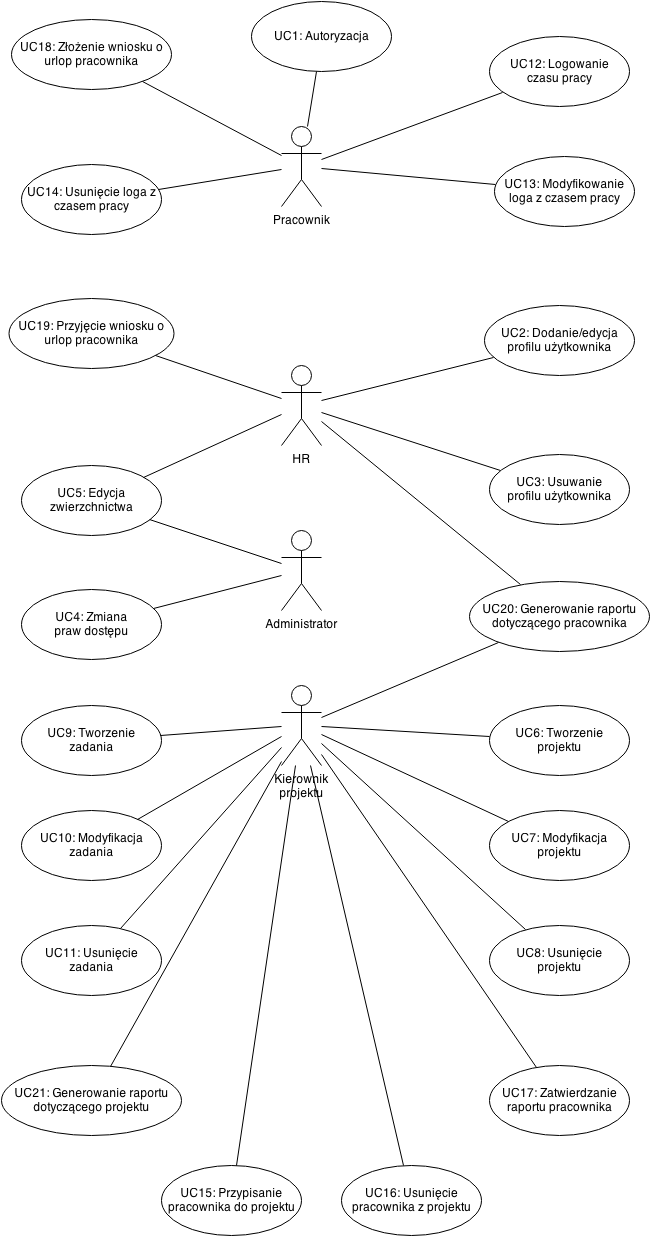
\includegraphics[scale=0.49]{diagramy/usecases/usecases.png}
    \caption{Diagram przypadków użycia}
    \label{fig:usecase}
\end{figure}
